%----------------------------------------------------------------------------
\chapter{A Train Benchmark}
%----------------------------------------------------------------------------

A Train Benchmark egy projekt, melynek célja adatbázisrendszerek teljesítményének mérése modellvalidációs forgatókönyvek használatával. A modellvalidációs forgatókönyv 4 fázisból épül fel: beolvasás, ellenőrzés, módosítás, újraellenőrzés. Beolvassuk a modellt, ellenőrizzük, hogy megfelelnek-e bizonyos előre meghatározott kényszernek, ezután eszközölünk rajta valamilyen módosítást (javítunk vagy rontunk a modellen), majd ismét elvégzünk rajta egy ellenőrzést. Ezalatt mérjük, hogy az adatbázis-rendszer milyen gyorsan végzi el ezeket a műveleteket, majd az eredményt összehasonlítjuk. 

\section{A Train Benchmark metamodell}

A metamodell egy absztrakt nyelv, mellyel a modellről írhatunk le információkat. Az itt szereplő metamodell meghatározza azt, hogy milyen típusú elemekről milyen információt tárolunk, ezenfelül leírja a közöttük lévő kapcsolatot is.

A Train Benchmark egy vasúti pályának az elemeit, azok tulajdonságait használja fel egy valós probléma szimulálására. A metamodell osztályokból épül fel, amik meghatározzák az adott elemnek az általunk fontos tulajdonságok összességét, ezeket tároljuk. Ezek az osztályok a következők:
\begin{itemize}
	\item \emph{RailwayElement}: Minden osztály ennek az osztálynak a leszármazottja. Egyetlen közös tulajdonságot, az egyedi azonosítót tartalmazza.
	\item \emph{Semaphore}: Jelzi a vonatnak, hogy az adott útszakaszon áthaladhat-e. Az aktuális állapotát tároljuk. (A továbbiakban: szemafor)
	\item \emph{TrackElement}: A sínpálya legkisebb számunkra fontos alkotóelemei, a \emph{Segment} és a \emph{Switch} ősosztálya.
	\item \emph{Segment}: Az útnak egy kisebb része, ami már megfigyelhető szenzorok által. A modellben szereplő tulajdonsága a hossza. (A továbbiakban: útszakasz)
	\item \emph{Switch}: Két útszakasz között helyezkedik el és meghatározza azt, hogy merre halad tovább a vonat, amikor ideér. (A továbbiakban váltó)
	\item \emph{Route}: Egy vasúti sínpár szakasza két szemafor között. útszakaszokból és váltókból áll össze. Azt tároljuk róla, hogy aktív-e, azaz, hogy az összes váltó olyan állásban van, hogy a vonat ezen az útvonalon halad végig. (A továbbiakban: út)
	\item \emph{Region}: Szenzorokat, útszakaszokat és váltókat magába foglaló konténer. (A továbbiakban régió)
	\item \emph{RailwayContainer}: Utakat és a régiókat tartalmazó konténer.
	\item \emph{Sensor}: A hozzá tartozó útszakaszokat, illetve váltókat monitorozza. (A továbbiakban: szenzor)
	\item \emph{SwitchPosition}: A váltó az úthoz mért relatív állását mutatja, azaz, hogy a váltónak merre kell állnia, hogy a szegmenseken végighaladó vonat az adott úton haladjon. 
\end{itemize}

\begin{figure}[H]
	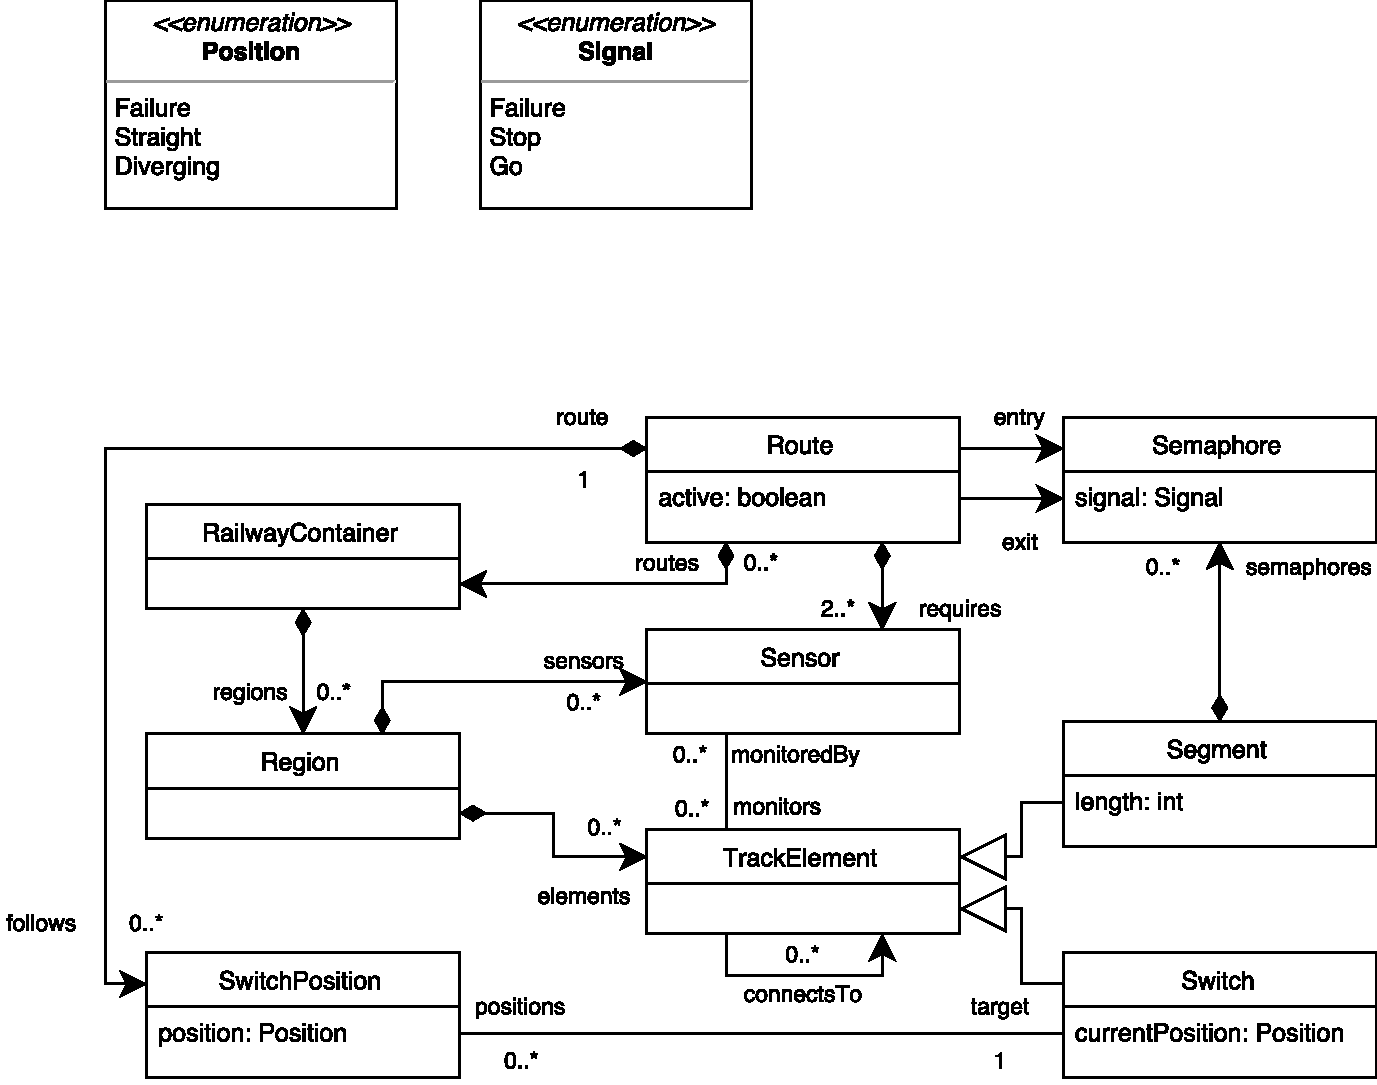
\includegraphics[width=\linewidth, keepaspectratio]{figures/model.pdf}
	\caption{A Train Benchmark modellje}
	\label{fig:ModelDiagram}
\end{figure}

\section{Kényszerek}

A Train Benchmarkban összesen 6 kényszer teljesülését követelik meg. Ezek között vannak olyan egyszerűek, mint a \emph{PosLength}, ami azt követeli meg, hogy egy szegmens hossza pozitív legyen, és vannak bonyolultabbak, mint a \emph{ConnectedSegment}, ami azt, hogy 6 egymást követő szegmenst ne felügyeljen egy szenzor. Ez utóbbi ellenőrzése egy olyan relációs adatbázisban, ahol minden osztályhoz egy tábla tartozik, 7 tábla összekapcsolását követeli meg.
Két kényszert valósítottunk meg, ezért ezt a kettőt mutatjuk be részletesebben.

\subsection{RouteSensor}

Az utak és a rajtuk található váltók között nincs közvetlen kapcsolat. Az utakhoz csak a \emph{SwitchPosition} kapcsolódik, egy \emph{SwitchPosition} pedig pontosan egy váltóhoz tartozik. Ezáltal, ha közvetve is, de egy úthoz a rajta található váltókat hozzá lehet rendelni. A \emph{RouteSensor} azt követeli meg, hogy az úton található váltókhoz ne tartozhasson szenzor úgy, hogy az út és a szenzor között ne legyen kapcsolat. A modellben ez a \ref{fig:RouteSensor} ábrán látható módon jelenik meg. Amennyiben a kérdőjellel ellátott él hiányzik, akkor a kényszer nem teljesül.

\begin{figure}[!ht]
	\centering
	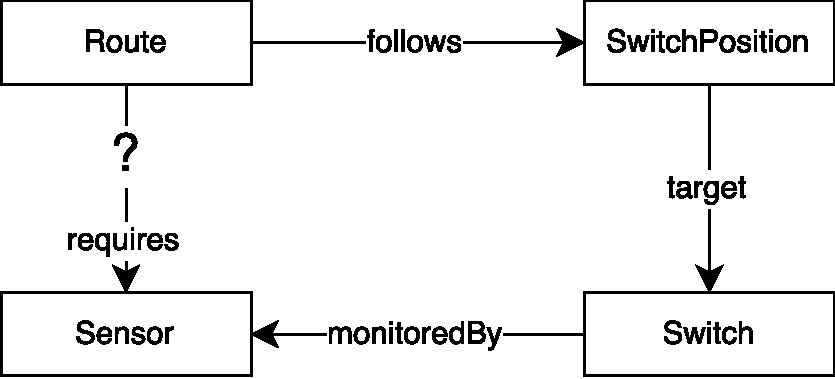
\includegraphics[width=0.7\linewidth, keepaspectratio]{figures/RouteSensor.pdf}
	\caption{A \emph{RouteSensor} kényszer}
	\label{fig:RouteSensor}
\end{figure}

\subsection{SwitchSet}

A \emph{SwitchSet} kényszer teljesülésének feltétele, hogy amikor egy út aktív és az elején található szemafor szabad jelzést ad, akkor az összes váltónak olyan állásban kell lennie, hogy a vonat az adott úton haladjon végig. Amennyiben nem így lenne, a vonat más útvonalon haladna végig, tehát nem lenne igaz, hogy az út aktív. A modellben ezt a \ref{fig:SwitchSet} ábrán szereplő elemek ellenőrzésével lehet észrevenni.

\begin{figure}[!ht]
	\centering
	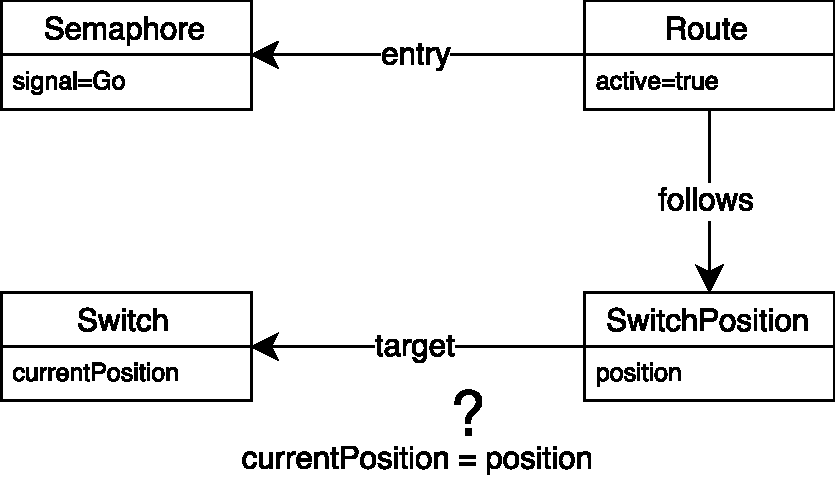
\includegraphics[width=0.7\linewidth, keepaspectratio]{figures/SwitchSet.pdf}
	\caption{A \emph{SwitchSet} kényszer}
	\label{fig:SwitchSet}
\end{figure}

%TODO Hiányzik innen egy bekezdés

\section{A fejlesztés lépései}

A valóságban egy ilyen modell folyamatosan bővül, azáltal, hogy új sínpályák építését-, a régiek felújítását tervezik. Ezáltal a számítógépes modellt is bővíteni kell, ami programozók feladata. Ilyen esetben előfordulnak hibák, amiket javítani kell. Ennek a szimulálására a Train Benchmark 3 különböző szcenáriót különböztet meg: \emph{Batch}, \emph{Inject}, \emph{Repair}.

\subsection{Batch}

Ebben az esetben azt szimulálja a Train Benchmark, hogy az adatbázisba betöltenek egy modellt és ellenőrzik a kényszereket. Ez a validáció első szakasza. A kiértékelés ezen szakaszának célja mérni, hogy milyen gyorsan lehet egy már kész modellt importálni és a kényszereket először. A további lépések folyamán lehet információnk arról, hogy a már az adatbázisban lévő adatok korábban mennyire feleltek meg a kényszereknek, azonban itt még nincs.

\subsection{Inject}

Az \emph{Inject} szakaszban véletlenszerű hibainjektálás történik a modellbe és minden ilyen után egy újraellenőrzés következik, majd ez a két lépés ciklikusan ismétlődik egy paraméter által meghatározott érték szerint. Ezáltal lehet mérni, ha egy modellben kis változtatásokat hajtanak végre, akkor az adott adatbázis-kezelő ezt milyen gyorsan végzi el. Képes-e a modell kis részét megváltoztatni vagy ilyenkor az egészen műveletet kell végezni. A hibainjektálás a különböző kényszerekhez más és más módon zajlik. A \emph{RouteSensor} megsértéséhez egy úthoz tartozó véletlenszerű \emph{requires} élet törlünk, a \emph{SwitchSet} megsértéséhez pedig a megfelelő váltó \emph{currentPosition} tulajdonságát érvénytelen értékre állítjuk.

\subsection{Repair}

Ebben a fázisban a hibák kijavításának szimulálása zajlik. Itt is a javítást követően a kényszerek ismételt ellenőrzése következik és hasonlóan az \emph{Inject} lépéshez, itt is több javítás-újraellenőrzés lépés van. A javításhoz a hibabeszúráshoz képest általában sokkal több erőforrásra van szükség, mivel itt először meg is kell keresni a hibát, és csak utána lehet kijavítani. Ezt a \emph{RouteSensor} esetében  a hiányzó \emph{requires} él pótlásával, a \emph{SwitchSet} esetében a váltó \emph{currentPosition}-jének a \emph{SwitchPosition} \emph{position}-jéhez való igazításával lehet megtenni.

\section{Resource Description Framework}

A \emph{Resource Description Framework} (\emph{RDF}) egy leíró keretrendszer, amelyet adatok reprezentálására alkalmas. Elsődleges célja számítógépek közötti információcsere, nem az emberi feldolgozás. Ez egy általános célú keretrendszer, ezáltal különböző alkalmazások között is alkalmas információcserére. Az \emph{RDF} adathármasokat (\emph{triple}) tárol, ami a következőkből épül fel:
\begin{itemize}
	\item \emph{subject}: Az adathármas alanya, rá vonatkozik a \emph{triple}-ben tárolt adat.
	\item \emph{predicate}: Tulajdonság, a \emph{subject} és az \emph{object} közötti kapcsolat típusát írja le.
	\item \emph{object}: A tulajdonság tárgya, leírhat egyszerű tulajdonságot is, de amennyiben a predicate két, a modellben szereplő elem kapcsolatának típusát jelöli, akkor egy másik modellbeli elemet fog jelenteni.
\end{itemize}

Ez alapján felfoghatjuk az \emph{RDF}-et úgy, mint egy irányított gráfot, melyeknek a csúcsain és élein információt tárolunk. A csúcsok a \emph{subject}-ek és \emph{object}-ek a csúcsok, a \emph{predicate}-ek pedig a köztük lévő élek. Többféle szintaxisa létezik, ebből a \emph{Turtle}-t emeljük ki, mert a Train Benchmark \emph{RDF} alapú eszközei ezt használják. A \emph{Turtle} a \emph{subject}-et, \emph{predicate}-et és \emph{object}-et szóközzel választja el egymástól és egy hármasnak a leírása ponttal végződik. Emellett lehetőség van egy \emph{subject}-ről több \emph{predicate}-et és \emph{object}-et tárolni úgy, hogy az első sor végére (melyben a \emph{subject} szerepel) pontosvesszőt teszünk, majd a további sorokban nem írjuk le fölöslegesen a \emph{subject}-et. Az ilyen felsorolás legvégére pontot kell tennünk.
%TODO: ábra
\begin{figure}[H]
	\centering
	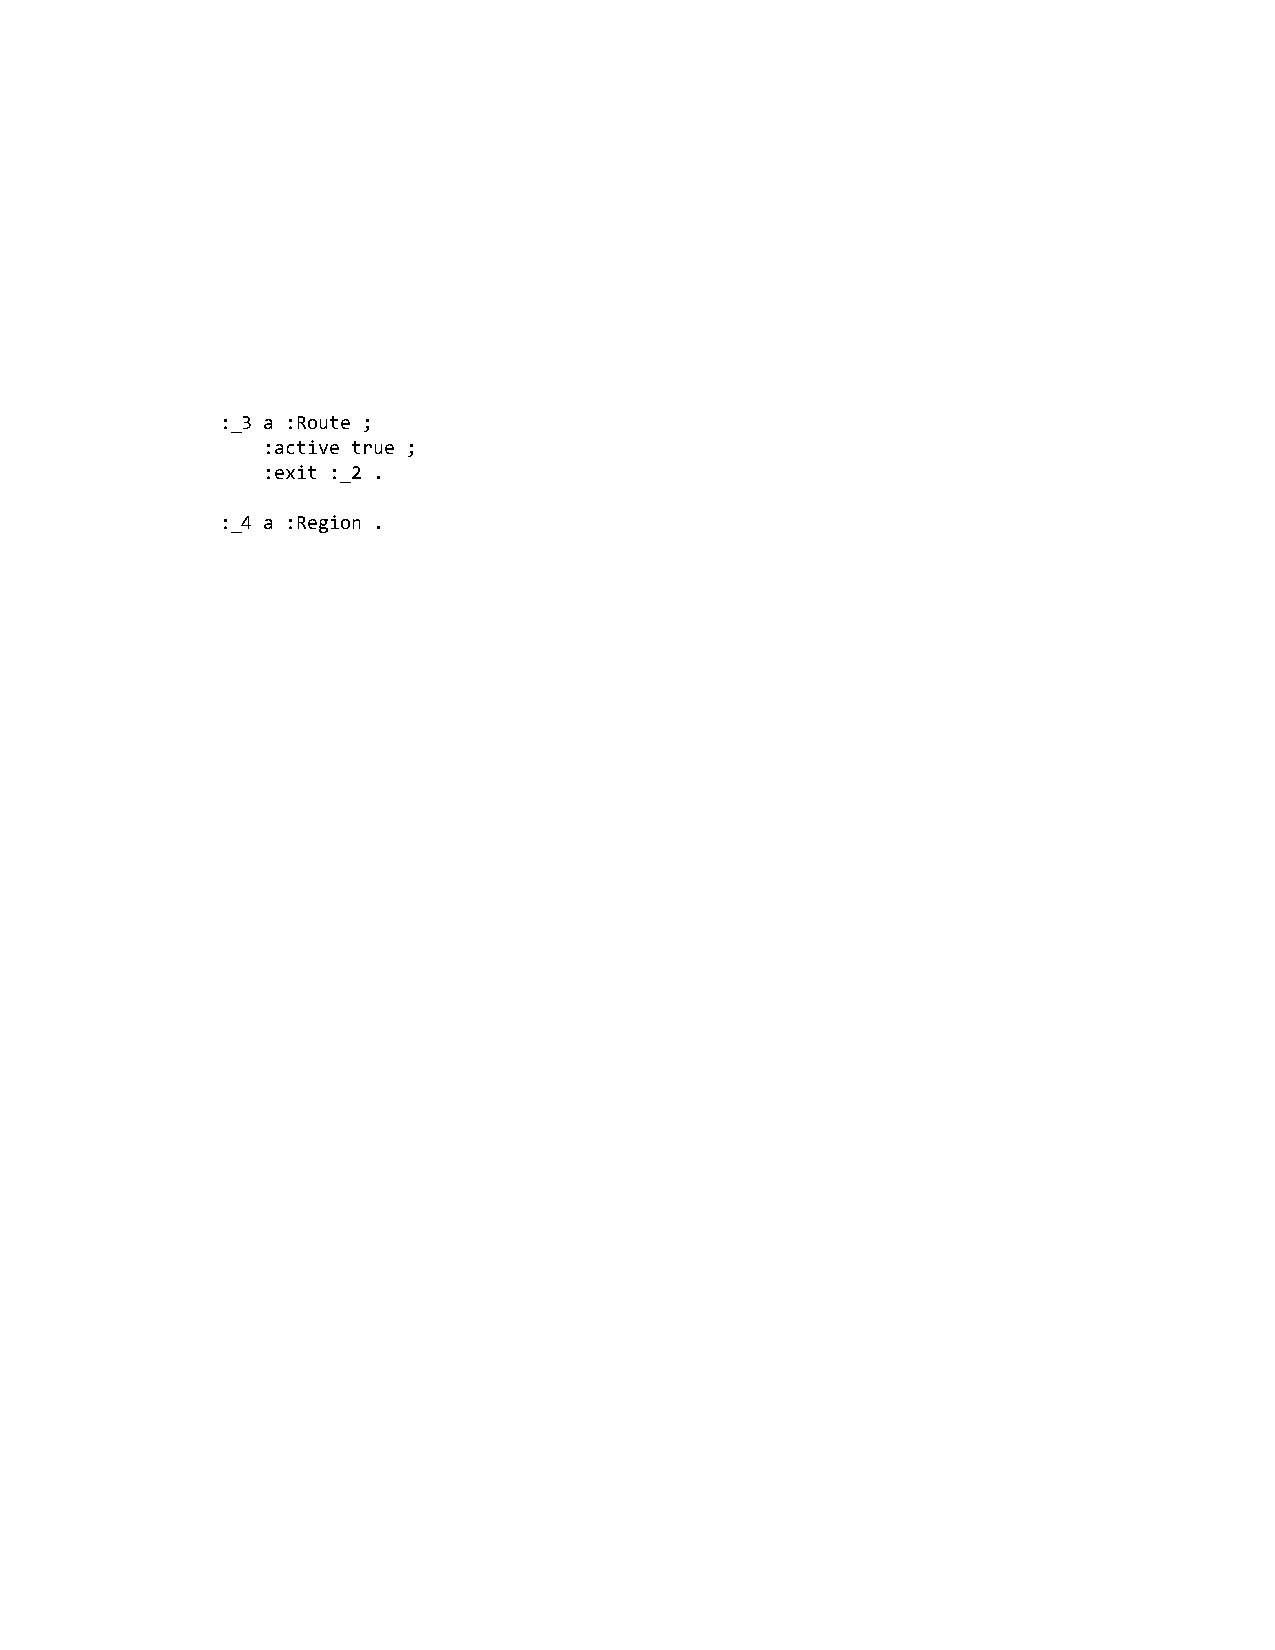
\includegraphics{figures/Turtle.pdf}
	\caption{Az egyik modell \emph{Turtle} leírásának részlete.}
	\label{fig:Turtle}
\end{figure}

A Train Benchmark modelljének leírása \emph{Turtle}-ben a \ref{fig:Turtle} ábrán látható. A \emph{subject} mindig egy szám, ami egy elem egyedi azonosítója, a \emph{RailwayElement} ősosztály egyetlen tulajdonsága. A \emph{predicate} meghatározza azt, hogy a \emph{triple} az elem típusát, tulajdonságát vagy két elem közötti kapcsolatot ír le. Amennyiben \texttt{a} az értéke, akkor a \emph{subject} egy típust fog leírni (például \emph{Route} vagy \emph{Semaphore}). Egy elem leírása mindig azzal kezdődik, hogy meghatározza a típusát. Ezután felsorolás-szerűen megadja a tulajdonságait (active vagy signal), mégpedig úgy, hogy a \emph{predicate} a tulajdonság nevét, az \emph{object} pedig az értékét. Ezután leírja az egyes elemek közötti kapcsolatot. Ebben az esetben a \emph{predicate} a kapcsolat neve, míg a \emph{subject} a cél objektum azonosítója. 



\section{Létező Train Benchmark implementációk}

A Train Benchmark 10 különböző eszközre készült el. Ezek között található a napjainkban legelterjedtebb relációs adatbázis-kezelő, \emph{Eclipse Modeling Framework}-öt használó, illetve \emph{RDF}-alapú és gráfadatbázis is. A dolgozat ezek közül az \emph{RDF}-alapú Jena és  RDF4J futtatását követelte meg.
Az \emph{RDF4J}-ben és a \emph{Jena}-ban az a közös, hogy mindkettő egy Java keretrendszer \emph{RDF} alapú adatok feldolgozására, lekérdezésére és módosítására. Mindkettő \emph{SPARQL} lekérdező nyelvet használ.